% % % % % % % % % % % % % % % % % % % % % % % % % % % % % % % % % % % % % % % %
% LaTeX4EI Template for Cheat Sheets                                Version 1.0
%
% Authors: Emanuel Regnath, Martin Zellner
% Contact: info@latex4ei.de
% Encode: UTF-8, tabwidth = 4, newline = LF
% % % % % % % % % % % % % % % % % % % % % % % % % % % % % % % % % % % % % % % %


% ======================================================================
% Document Settings
% ======================================================================

% possible options: color/nocolor, english/german, threecolumn
% defaults: color, english
\documentclass[english]{latex4ei/latex4ei_sheet}

% set document information
\title{Signal Processing and\\ Machine Learning}
\author{LaTeX4EI}					% optional, delete if unchanged
\myemail{info@latex4ei.de}			% optional, delete if unchanged
\mywebsite{www.latex4ei.de}			% optional, delete if unchanged


%\DeclareMathOperator{\T}{\textsf{\textit{T}}}		% Zufallsvariable X
\DeclareMathOperator{\Bias}{Bias}		% Zufallsvariable X
\DeclareMathOperator{\argmax}{argmax}

\DeclareMathOperator{\rang}{rang}
\renewcommand{\vec}[1]{\underline{\boldsymbol{#1}}}
%\renewcommand{\vec}[1]{\boldsymbol{#1}}



\newcommand{\x}{\textit{x}}
\newcommand{\vx}{\underline{\textbf{\textit{x}}}}
\newcommand{\VX}{\underline{\textbf{\textit{X}}}}

\newcommand{\y}{\textit{y}}
\newcommand{\vy}{\underline{\textbf{\textit{y}}}}
\newcommand{\VY}{\underline{\textbf{\textit{Y}}}}


\newcommand{\VA}{\underline{\textit{A}}}
\newcommand{\A}{\textit{A}}
\newcommand{\va}{\underline{\textbf{\textit{a}}}}

\newcommand{\VB}{\underline{\textit{B}}}




% ======================================================================
% Begin
% ======================================================================
\begin{document}

\IfFileExists{git.id}{\input{git.id}}{}
\ifdefined\GitRevision\mydate{\GitNiceDate\ (git \GitRevision)}\fi
% Title
% ----------------------------------------------------------------------
\maketitle   % requires ./img/Logo.pdf


% Section
% ----------------------------------------------------------------------
\section{Math}
% ======================================================================

\begin{sectionbox}
	\begin{tabular}{@{}llll}
		$\pi \approx \num{3,14159}$ & $e \approx \num{2,71828}$ & $\sqrt{2} \approx \num{1,414}$ & $\sqrt{3} \approx \num{1,732}$ \\
	\end{tabular}

	\textbf{Binome, Trinome}\\
	$(a\pm b)^2 = a^2 \pm 2ab + b^2$ \hfill $a^2 - b^2 = (a-b)(a+b)$\\
	$(a \pm b)^3 = a^3 \pm 3a^2b + 3ab^2 \pm b^3$\\
	$(a+b+c)^2 = a^2 + b^2 + c^2 + 2ab + 2ac + 2bc$
	\\[0.5em]
	\textbf{Folgen und Reihen}\\
	$\underset{\text{Aritmetrische Summenformel}}{\sum \limits_{k=1}^{n} k = \frac{n (n+1)}{2}}$ \quad $\underset{\text{Geometrische Summenformel}}{\sum \limits_{k=0}^{n} q^k = \frac{1 - q^{n+1}}{1-q}}$ \quad $\underset{\text{Exponentialreihe}}{\sum\limits_{n = 0}^{\infty} \frac{\cx z^n}{n!} = e^{\cx z}}$\\
	\\[0.5em]
	\textbf{Mittelwerte} \quad ($\sum$ von $i$ bis $N$) \hfill {\small (Median: Mitte einer geordneten Liste)}\\
	\begin{tabular*}{\columnwidth}{@{\extracolsep\fill}l@{\quad\ $\ge$}l@{\quad\ $\ge$}l}
	$\underset{\text{Arithmetisches}}{\ol x_{\ir{ar}} = \frac{1}{N} \sum x_i}$ & $\underset{\text{Geometrisches Mittel}}{\ol x_{\ir{geo}} = \sqrt[N]{ \prod x_i }}$ & $\underset{\text{Harmonisches}}{\ol x_{\ir hm} = }\frac{N}{\sum \frac{1}{x_i}}$\\
	\end{tabular*}
	\\[0.5em]
	\textbf{Ungleichungen:} \hfill Bernoulli-Ungleichung:  $(1+x)^n \ge 1+nx$\\
	$\underset{\text{Dreiecksungleichung}}{\big|\! \abs{x}- \abs{y}\!\big| \le \abs{x \pm y} \le \abs{x} + \abs{y}}$ \hfill
	$\underset{\text{Cauchy-Schwarz-Ungleichung}}{\left| \vec x^\top \bdot \vec y \right| \le \| \vec x\| \cdot \| \vec y\|}$
	\\[0.5em]
	\textbf{Mengen:} De Morgan: $\overline{A \capdot B} = \overline{A} \cupplus \overline{B}$ \hfill $\overline{A \cupplus B} = \overline{A} \capdot \overline{B}$
\end{sectionbox}

\begin{sectionbox}
	\subsection[Exp. und Log.]{Exp. und Log.\ \ $e^x := \lim\limits_{n \rightarrow \infty} \left( 1 + \frac{x}{n} \right)^n \hfill e \approx 2,71828$}
	\begin{tabular*}{\columnwidth}{@{\extracolsep\fill}lll@{}}
		$a^x = e^{x \ln a}$ & $\log_a x = \frac{\ln x}{\ln a}$ & $\ln x \le x -1$\\
		$\ln(x^{a}) = a \ln(x)$ & $\ln(\frac{x}{a}) = \ln x - \ln a$ & $\log(1) = 0$\\
	\end{tabular*}
\end{sectionbox}


\begin{sectionbox}
	\subsection[Matrizen]{Matrizen $\ma A \in\mathbb{K}^{m \times n}$}
	$\ma A=(a_{ij}) \in \mathbb K^{m\times n}$ hat $m$ Zeilen (Index $i$) und $n$ Spalten (Index $j$)
	\begin{tabular*}{\columnwidth}{ll}
	$(\ma A + \ma B)^\top = \ma A^\top + \ma B^\top$ & $(\ma A \cdot \ma B)^\top = \ma B^\top \cdot \ma A^\top$\\
	${(\ma A^\top)}^{-1} = {(\ma A^{-1})}^\top$ & $(\ma A \cdot \ma B)^{-1} = \ma B^{-1}\ma A^{-1}$
	\end{tabular*}
	$\dim \mathbb K = n = \rang\ma A + \dim\ker\ma A$ \qquad $\rang\ma A = \rang\ma A^\top$


	\subsubsection{Quadratische Matrizen $A \in \mathbb{K}^{n \times n}$}
	regulär/invertierbar/nicht-singulär $\Leftrightarrow \det (\ma A) \ne 0 \Leftrightarrow \rang\ma A = n$\\
	singulär/nicht-invertierbar $\Leftrightarrow \det (\ma A) = 0 \Leftrightarrow \rang\ma A \ne n$\\
	orthogonal $\Leftrightarrow \ma A^\top=\ma A^{-1} \Ra \det(\ma A) = \pm 1$\\
	symmetrisch: $\ma A=\ma A^\top$ \qquad schiefsymmetrisch: $\ma A=-\ma A^\top$
	%\item hermitsch: $\ma A=\overline{\ma A}^\top$, unitär:$\ma A^{-1} = \overline{\ma A}^\top$


	\subsubsection[Determinante]{Determinante von $\ma A\in \mathbb K^{n\times n}$: $\det(\ma A)=|\ma A|$}
	$\det\mat{ \ma A & \ma 0 \\ \ma C& \ma D }= \det\mat{ \ma A & \ma B \\ \ma 0 & \ma D } = \det(\ma A)\det(\ma D)$ \\
	\begin{tabular*}{\columnwidth}{@{\extracolsep\fill}ll}
	$\det(\ma A) = \det(\ma A^T)$ & $\det(\ma A^{-1}) = \det(\ma A)^{-1}$
	\end{tabular*}
	$\det(\ma A\ma B) = \det(\ma A)\det(\ma B) = \det(\ma B)\det(\ma A) = \det(\ma B\ma A)$\\
	Hat $\ma A$ 2 linear abhäng. Zeilen/Spalten $\Rightarrow |\ma A|=0$ \\

	\subsubsection{Eigenwerte (EW) $\lambda$ und Eigenvektoren (EV) $\underline v$}
	\begin{emphbox}
		\large $\ma A \vec v = \lambda \vec v$ \quad\ $\det \ma A = \prod \lambda_i$ \quad\ $\Sp \ma A = \sum a_{ii} = \sum \lambda_i$
	\end{emphbox}
	Eigenwerte: $\det(\ma A - \lambda \ma 1) = 0$ Eigenvektoren: $\ker(\ma A - \lambda_i \ma 1) = \vec v_i$\\
	EW von Dreieck/Diagonal Matrizen sind die Elem. der Hauptdiagonale.


	\subsubsection{Spezialfall $2 \times 2$ Matrix $A$}
	\parbox{3cm}{ $\det(\ma A) = ad-bc$ \\ $\Sp(\ma A) = a+d$ } $\mat{a & b\\ c & d}^{-1} = \frac{1}{\det \ma A} \mat{d & -b\\ -c& a}$\\
	$\lambda_{1/2} = \frac{\Sp \ma A}{2} \pm \sqrt{ \left( \frac{\mathrm{sp} \ma A}{2} \right)^2 - \det \ma A }$

	\subsubsection{Differentiation}
	$\frac{\partial \vec x^\top \vec y}{\partial \vec x} = \frac{\partial \vec y^\top \vec x}{\partial \vec x} = \vec y$\qquad
	$\frac{\partial \vec x^\top \ma A \vec x}{\partial \vec x} = (\ma A + \ma A^\top)\vec x$ \\
	$\frac{\partial \vec x^\top \ma A \vec y}{\partial \ma A} = \vec x \vec y^\top$ \qquad $\frac{\partial \det( \ma B \ma A \ma C )}{\partial \ma A} = \det(\ma B \ma A \ma C) \left( \ma A^{-1} \right)^\top$
\end{sectionbox}



\begin{sectionbox}
	\subsubsection{Ableitungsregeln ($\forall \lambda, \mu \in \mathbb R$)}
	\begin{tabular}{@{}l@{\quad}ll@{}}
		Linearität: & $(\lambda f + \mu g)' (x) = \lambda f'(x) + \mu g'(x_0)$  \\
		Produkt: & $(f \cdot g)'(x) = f'(x) g(x) + f(x) g'(x)$\\
		Quotient: & $\left(\frac{f}{g}\right)' (x) = \frac{g(x)f'(x) -f(x) g'(x)}{g(x)^2}$ \quad $\left(\frac{\text{NAZ}-\text{ZAN}}{\text{N}^2}\right)$\\
		Kettenregel & $\left( f\bigl(g(x)\bigr) \right)' = f'\bigl(g(x)\bigr) g'(x)$\\
	\end{tabular}
\end{sectionbox}

\begin{sectionbox}
	\subsection{Integrale $\int e^x\mathrm dx = e^x = (e^x)'$}
	%$\int_a^b f(x) \mathrm dx = F(b) - F(a)$\\
	\begin{tabular*}{\columnwidth}{ll}
	Partielle Integration: & $\int uw'=uw-\int u'w$\\
	Substitution: & $\int f(g(x)) g'(x)\diff x=\int f(t)\diff t$
	\end{tabular*}
	\begin{tablebox}{@{\hspace{5mm}}c@{\extracolsep\fill}c@{\extracolsep\fill}c@{\hspace{5mm}}}
		$F(x) - C$ & $f(x)$ & $f'(x)$ \\ \cmrule
		$\frac{1}{q+1}x^{q+1}$ & $x^q$ & $qx^{q-1}$ \\[1em]
		\raisebox{-0.2em}{$\frac{2\sqrt{ax^3}}{3}$} & $\sqrt{ax}$ & \raisebox{0.2em}{$\frac{a}{2\sqrt{ax}}$}\\
		$x\ln(ax) -x$ & $\ln(ax)$ & $\textstyle \frac{1}{x}$\\
		$\frac{1}{a^2} e^{ax}(ax- 1)$ & $x \cdot e^{ax}$ & $e^{ax}(ax+1)$ \\
		$\frac{a^x}{\ln(a)}$ & $a^x$ & $a^x \ln(a)$ \\
		$-\cos(x)$ & $\sin(x)$ & $\cos(x)$\\
		$\cosh(x)$ & $\sinh(x)$ & $\cosh(x)$\\
		$-\ln |\cos(x)|$ & $\tan(x)$ & $\frac{1}{\cos^2(x)}$ \\
	\end{tablebox}

	\begin{tabular*}{\columnwidth}{ll}
	\multicolumn{2}{c}{$\int e^{at} \sin(bt) \diff t = e^{at} \frac{a \sin(bt) + b \cos(bt)}{a^2 + b^2}$}\\
	$\int \frac{\diff t}{\sqrt{at+b}} = \frac{2 \sqrt{at+b}}{a}$ & $\int t^2 e^{at} \diff t = \frac{(ax-1)^2+1}{a^3} e^{at}$\\
	$\int t e^{at} \diff t = \frac{at-1}{a^2} e^{at}$ & $\int x e^{ax^2} \diff x = \frac{1}{2a} e^{ax^2}$\\
	\end{tabular*}

	\subsubsection{Volumen und Oberfläche von Rotationskörpern um $x$-Achse}
	$V = \pi \int_a^b f(x)^2 \mathrm dx$ \qquad \quad $O = 2 \pi \int_a^b f(x) \sqrt{1 + f'(x)^2} \mathrm dx$
\end{sectionbox}


% Section
% ----------------------------------------------------------------------
\section{Probability Theory Basics}
% ======================================================================


\begin{sectionbox}
	\subsection{Kombinatorik}
	Mögliche Variationen/Kombinationen um $k$ Elemente von maximal $n$ Elementen zu wählen bzw. $k$ Elemente auf $n$ Felder zu verteilen:\\
	\begin{tablebox}{l|cc}
		& \large Mit Reihenfolge & \large Reihenfolge egal\\ \cmrule
		%& ungleiche Elemente & gleiche Elemente \\
		\large Mit Wiederholung & \large $n^k$ & \Large $\binom{n+k-1}{k}$\\[0.2em]
		\large Ohne Wiederholung & \Large $\frac{n!}{(n-k)!}$ & \Large $\binom nk$\\
	\end{tablebox}
	Permutation von $n$ mit jeweils $k$ gleichen Elementen: $\frac{n!}{k_1 ! \cdot k_2 ! \cdot ...}$\\
	Binomialkoeffizient $\binom nk = \binom n{n-k} = \frac{n!}{k! \cdot (n-k)!}$\\
	$\binom n0 = 1$ \quad $\binom n1 = n$ \quad $\binom 42 = 6$ \quad $\binom 52 = 10$ \quad $\binom 62 = 15$
\end{sectionbox}


\begin{sectionbox}
	\subsection{Der Wahrscheinlichkeitsraum $(\Omega,\mathbb F,\P)$}
	\begin{tablebox}{lll}
		\textbf{Ergebnismenge} & $\Omega = \eset{\omega_1,\omega_2, ...}$ & Ergebnis $\omega_j \in \Omega$\\[0.5em]
		\textbf{Ereignisalgebra} & $\mathbb F = \eset{A_1,A_2,...}$ & Ereignis $A_i \subseteq \Omega$\\
		\textbf{Wahrscheinlichkeitsmaß} & $\P:\mathbb F \ra [0,1]$ & $\P(A) = \frac{|A|}{|\Omega|}$\\
	\end{tablebox}
\end{sectionbox}


\begin{sectionbox}
	\subsection{Wahrscheinlichkeitsmaß $\P$}
	$\P(A) = \frac{|A|}{|\Omega|}$ \hfill $\P(A \cup B) = \P(A) + \P(B) - \P(A \cap B)$\\
	\subsubsection{Axiome von Kolmogorow}
	\begin{tabular}{ll}
		Nichtnegativität: & $\P(A) \geq 0 \Ra \P:\mathbb F \mapsto [0,1]$ \\
		Normiertheit: & $\P(\Omega) = 1$ \\
		Additivität: & $\P\left(\bigcup\limits_{i=1}^{\infty} A_i \right) = \sum\limits_{i=1}^{\infty} \P(A_i)$, \\
		& wenn $A_i \cap A_j = \emptyset$, $\forall i \neq j$ \\
	\end{tabular}
\end{sectionbox}

\begin{sectionbox}
	\subsection{Bedingte Wahrscheinlichkeit}
	Bedingte Wahrscheinlichkeit für $A$ falls $B$ bereits eingetreten ist:\\
	$\P_B(A) = \P(A|B) = \frac{\P(A \cap B)}{\P(B)}$ %\qquad\quad $\P(B|A) = \P(A|B) \frac{\P(B)}{\P(A)}$\\

	\subsubsection{Totale Wahrscheinlichkeit und Satz von Bayes}
	Es muss gelten: $\bigcup\limits_{i \in I} B_i = \Omega$ für $B_i \cap B_j = \emptyset$, $\forall i \neq j$ \\
	\begin{tabular}{ll}
		Totale Wahrscheinlichkeit: & $\P(A) = \sum\limits_{i \in I} \P(A|B_i)\P(B_i)$\\
		Satz von Bayes: & $\P(B_k | A) = \frac{\P(A | B_k)\P(B_k)}{\sum\limits_{i \in I} \P(A|B_i) \P(B_i)}$\\
	\end{tabular}

	\textbf{Multiplikationssatz:} 	$\P(A \cap B) = \P(A|B)\P(B) = \P(B|A)\P(A)$
\end{sectionbox}

\begin{sectionbox}
	\subsection{Distribution}
		\begin{tablebox}{lll}
			Bezeichnung  & Abk. & Zusammenhang\\ \cmrule
	Wahrscheinlichkeitsdichte & pdf & $f_{\X}(x) = \frac{\diff F_{\X}(x)}{\diff x}$\\
	Kumulative Verteilungsfkt. & cdf & $F_{\X}(x) = \int\limits_{-\infty}^{x}{f_{\X}(\xi)\diff\xi}$ \\
		\end{tablebox}
	Joint CDF: $F_{\X,\Y}(x,y) = \P(\{\X \le x, \Y \le y\})$
\end{sectionbox}

\begin{sectionbox}
	\subsection[Relations]{Relations between $f_{\X}(x), f_{\X,\Y}(x,y), f_{\X|\Y}(x|y)$}
	\begin{emphbox}
		$\underset{\text{Joint PDF}}{f_{\X,\Y}(x,y)} = f_{\X|\Y}(x,y) f_{\Y}(y) = f_{\Y|\X}(y,x) f_{\X}(x)$\\
		$\underbrace{\int\limits_{-\infty}^{\infty} f_{\X,\Y}(x,ξ) \diff ξ}_{\text{Marginalization}} = \underbrace{\int\limits_{-\infty}^{\infty} f_{\X|\Y}(x,ξ)f_{\Y}(ξ) \diff ξ}_{\text{Total Probability}} = f_{\X}(x)$
	\end{emphbox}
\end{sectionbox}

\begin{sectionbox}
	\subsection{Bedingte Zufallsvariablen}
	\begin{tabular}{ll}
		Ereignis A gegeben: & $F_{\X|A}(x|A) = \P\left(\eset{\X \le x} | A\right)$\\
		ZV $\Y$ gegeben: & $F_{\X|\Y}(x|y)= \P\left(\eset{\X \le x} | \eset{\Y = y}\right)$\\
		& $p_{\X|\Y}(x|y) = \frac{p_{\X,\Y}(x,y)}{p_{\Y}(y)}$\\
		& $f_{\X|\Y}(x|y) = \frac{f_{\X,\Y}(x,y)}{f_{\Y}(y)} = \frac{\diff F_{X|Y}(x|y)}{\diff x}$\\
	\end{tabular}

\end{sectionbox}

\begin{sectionbox}
	\subsection{Unabhängigkeit von Zufallsvariablen}
	$\X_1,\shdots,\X_n$ sind stochastisch unabhängig, wenn für jedes $\vec{x} \in \R^n$ gilt:\\
	\begin{tabular}{l}
		$F_{\X_1,\shdots,\X_n}(x_1,\shdots,x_n) = \prod\limits_{i=1}^{n}{F_{\X_i}(x_i)}$\\
		$p_{\X_1,\shdots,\X_n}(x_1,\shdots,x_n) = \prod\limits_{i=1}^{n}{p_{\X_i}(x_i)}$\\
		$f_{\X_1,\shdots,\X_n}(x_1,\shdots,x_n) = \prod\limits_{i=1}^{n}{f_{\X_i}(x_i)}$\\
	\end{tabular}
\end{sectionbox}


% Section
% ----------------------------------------------------------------------
\section{Gaussian Stuff}

\begin{sectionbox}
	\subsection{Gaussian Channel}
	Channel: $\Y = h s_i + \textit N$ with $h \sim \mathcal N, \textit N \sim \mathcal N$\\
	$L(y_1,...,y_N) = \prod\limits_{i=1}^n f_{\Y_i}(y_i, h)$\\
	$f_{\Y_i}(y_i, h) = \frac{1}{\sqrt{2 \pi} \sigma}\exp\left( - \frac{1}{2 \sigma^2} (y_i - hs_i)^2 \right)$\\
	$\hat h_{ML} = \underset{h}{\operatorname{argmin}} \{\norm{\vec y - h \vec s}^2 \} = \frac{\vec s^\top \vec y}{\vec s^\top \vec s}$\\
	\\
	If multidimensional channel: $\vec y = \ma S \vec h + \vec n$:\\
	$L(\vec y, \vec h) =  \frac{1}{\sqrt{\det(2 \pi \ma C)}}\exp\left( - \frac{1}{2} (\vec y - \ma S \vec h)^\top\ma C^{-1}(\vec y - \ma S \vec h) \right)$\\
	$l(\vec y, \vec h) =  \frac{1}{2} \left( \log(\det(2 \pi \ma C) - (\vec y - \ma S \vec h)^\top\ma C^{-1}(\vec y - \ma S \vec h) \right)$\\
	\\
	$\frac{\diff}{\diff h} (\vec y - \ma S \vec h)^\top\ma C^{-1}(\vec y - \ma S \vec h) = −2 \ma S^\top \ma C^{−1}(\vec y − \ma S\vec h)$


	\textbf{Gaussian Covariance:} if $\Y \sim \mathcal N(0,σ^2), \textit N \sim \mathcal N(0,σ^2)$:\\
	$\ma C_{\Y} = \Cov[\Y,\Y] = \E[(\Y-μ)(\Y-μ)^\top] = \E[\Y\Y^\top]$\\
	For Channel $\Y = S h + \textit N$: $\E[\Y\Y^\top] = S\E[h h^\top]S^\top + \E[\textit N \textit N^\top]$
\end{sectionbox}


\begin{sectionbox}
	\subsection{Multivariate Gaussian Distributions}
	A vector $\vx$ of $n$ independent Gaussian random variables $\x_i$ is jointly Gaussian.
	If $\vx \sim \mathcal N(\vec \mu_{\vx}, \ma C_{\vx})$:\\
	\begin{emphbox}
		$f_{\vx}(\vec x) = f_{\x_1,...,\x_n}(\x_1,...,\x_n) =$ \\[1em] $= \frac{1}{\sqrt{\det(2 π \ma C_{\vx})}} \exp \left( - \frac{1}{2}\left(\vec x - \vec {μ}_{\vx}\right)^\top \ma C_{\vx}^{-1}\left(\vec x - \vec {μ}_{\vx}\right) \right)$\\
	\end{emphbox}

	Affine transformations $\vy = \ma A \vx + \vec b$ are jointly Gaussian with\\
	$\vy \sim \mathcal N(\ma A \vec \mu_{\vx} + \vec b, \ma A \ma C_{\vx} \ma A^\top) $\\
	All marginal PDFs are Gaussian as well

	\textbf{Contour Lines}\\
	Ellipsoid with central point $\E[\vec y]$ and main axis are the eigenvectors of $\ma C_{\vec y}^{-1}$\\

	\subsection{Conditional Gaussian}
	$\VA\!\sim\!\mathcal N(\vec {μ}_{\VA}, \ma C_{\VA}), \VB\!\sim\!\mathcal N(\vec{μ}_{\VB}, \ma C_{\VB})$ \\
		$\Ra (\VA| \VB\!=\!b) \sim \mathcal N(\vec{μ}_{\VA|\VB},\ma C_{\VA|\VB})$\\
	\\
	\textbf{Conditional Mean:}\\
	$\E[\VA|\VB = \vec b] = \vec{μ}_{\VA|\VB=\vec b} = \vec{μ}_{\VA} + \ma C_{\VA\VB}\;\ma C_{\VB\VB}^{-1} \left(\vec b - \vec{μ}_{\VB} \right)$\\
	\\
	\textbf{Conditional Variance:}\\
	$\ma C_{\VA|\VB} = \ma C_{\VA\VA} - \ma C_{\VA\VB}\;\ma C_{\VB\VB}^{-1}\;\ma C_{\VB\VA}$
\end{sectionbox}



\begin{sectionbox}
	\subsection{Misc}
	If CDF of gaussian distribution given $Φ(z) \sim \mathcal N(0,1)$ then for $\X \sim \mathcal N(1,1)$ the CDF is given as $Φ(x - μ_x)$
\end{sectionbox}

% Section
% ----------------------------------------------------------------------
\section{Common Distributions}
% ======================================================================

\begin{sectionbox}
	\subsection{Binomialverteilung $\mathcal B(n,p)$ mit $p \in [0,1], n \in \N$}
	Folge von $n$ Bernoulli-Experimenten\\
	$p$: Wahrscheinlichkeit für Erfolg \qquad $k$: Anzahl der Erfolge \\
	\\
	$p_{\X}(k) = B_{n,p}(k) = \begin{cases}
	\binom{n}{k} p^k (1 - p)^{n - k} & k \in \left\{0,\dots,n\right\} \\
	0 & \text{sonst} \\
	\end{cases}$
	\\
	\everymath{\displaystyle}
	\begin{tablebox}{l@{\extracolsep\fill}ll}
		$\underset{\text{Erwartungswert}}{\E[\X] =n p}\quad $ & $\underset{\text{Varianz}}{\Var[\X] =np (1-p)}$ & $\underset{\text{Wahrscheinlichkeitserz. Funktion}}{G_X (z) = (pz + 1 -p)^n}$\\
	\end{tablebox}
\end{sectionbox}

\begin{sectionbox}
	\subsection{Normalverteilung}
		\parbox{3.3cm}{\emph{WDF/PDF:} \\ 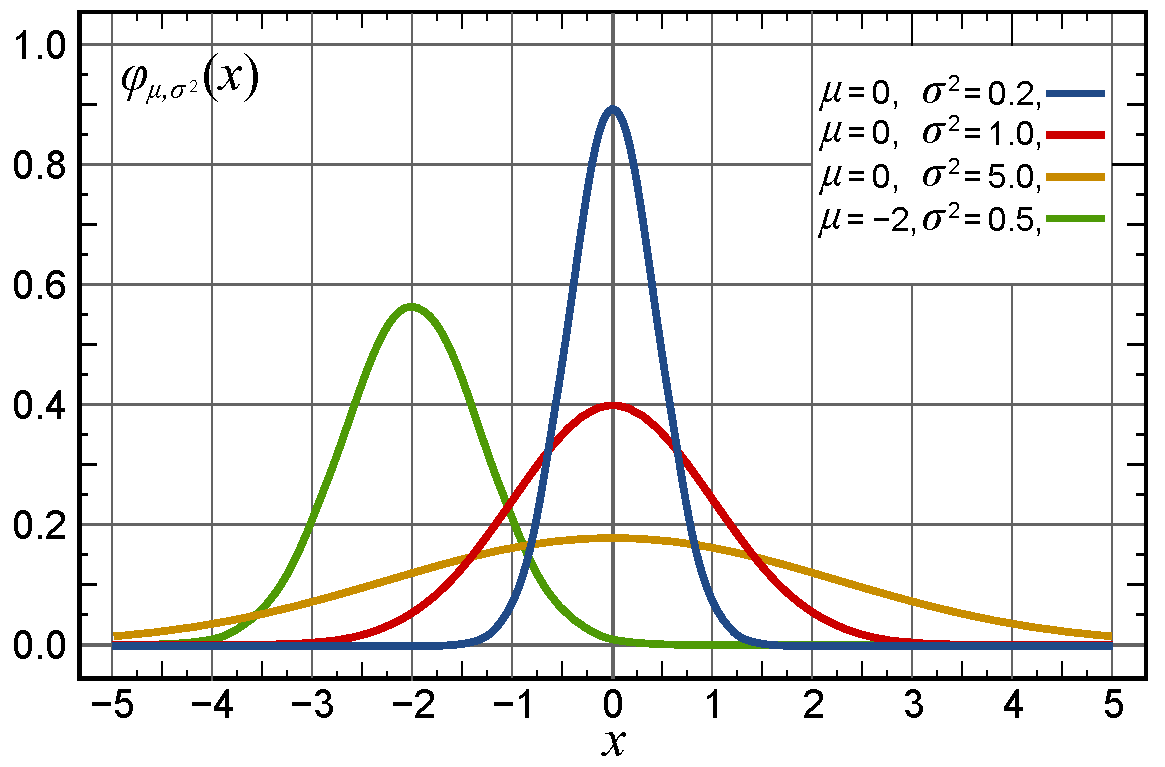
\includegraphics[width = 3.3cm]{./img/normal_pdf.pdf}}
		\parbox{3.3cm}{\emph{KVF/CDF:} \\ 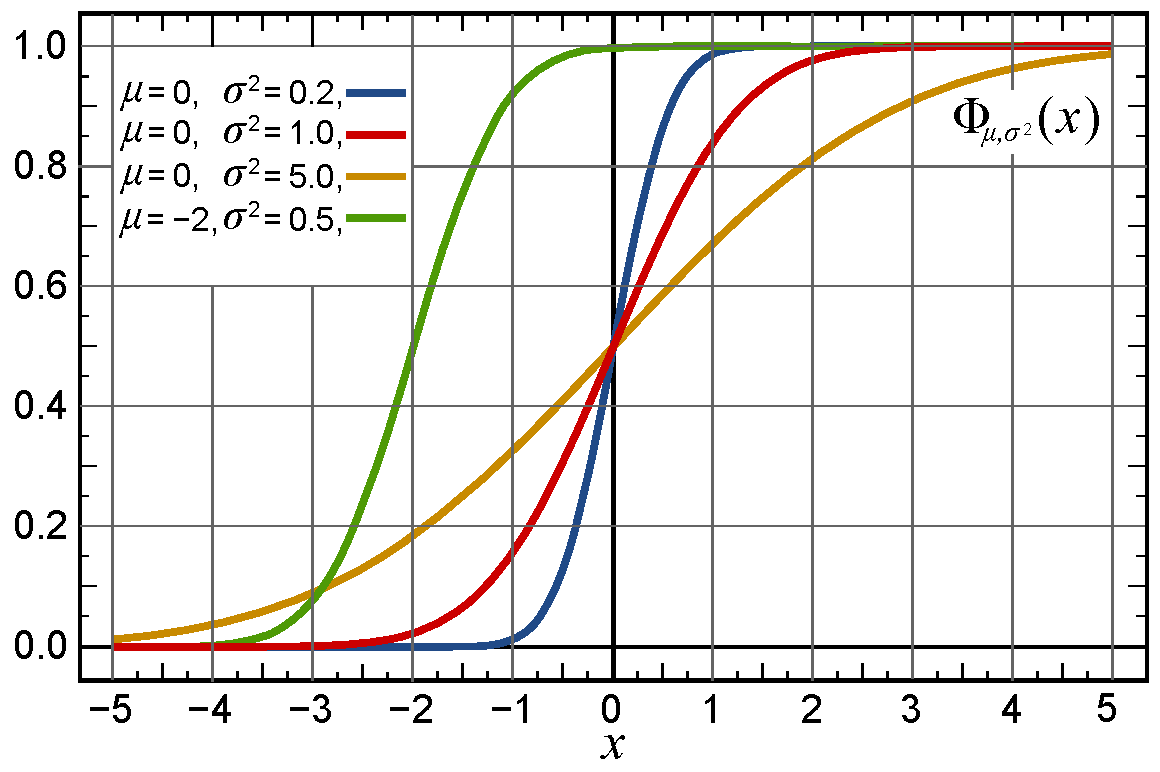
\includegraphics[width = 3.3cm]{./img/normal_cdf.pdf}}
		\textbf{WDF: }
		\boxed{f_X (x) = \frac{1}{\sqrt{2 \pi \sigma^2}} e^{-\frac{(x-\mu)^2}{2 \sigma^2}} \quad x \in \mathbb R} \qquad \parbox{1.2cm}{$\mu \in \mathbb R$ \\[0.5em] $\sigma > 0$}

		\begin{tablebox}{lll}
		\everymath{\displaystyle}
			$\underset{\text{Erwartungswert}}{\E(\X) = \mu}$ & $\underset{\text{Varianz}}{\Var(\X) =\sigma^2}$ & $\underset{\text{Charakt. Funktion}}{\varphi_{\X}(\omega) = e^{j\omega\mu-\frac{\omega^2\sigma^2}{2}}}$\\
		\end{tablebox} \everymath{\textstyle}
\end{sectionbox}

\begin{sectionbox}
	\subsection{Sonstiges}
	\textbf{Gammadistribution} $Γ(α,β)$: $\E[\X] = \frac{α}{β}$\\
	\textbf{Exponential:} $f(x,λ) = λ e^{-λx}$ \quad $\E[\X] = λ^{-1}$ \quad $\Var[\X] = λ^{-2}$
\end{sectionbox}

% Section
% ----------------------------------------------------------------------
\section{Wichtige Parameter}
% ======================================================================
\begin{sectionbox}
	\subsection{Erwartungswert (1. zentrales Moment)}
	gibt den mittleren Wert einer Zufallsvariablen an

	\begin{emphbox}
		$μ_{\X} = \E [\X] = \underset{\text{diskrete} \X:\Omega \ra \Omega'}{\sum\limits_{x \in \Omega'} x \cdot \P_{\X}(x)} \quad \stackrel{\wedge}{=}\quad \underset{\text{stetige} \X: \Omega \ra \R}{\int \limits_{\R} x \cdot f_{\X} (x) \diff x}$
	\end{emphbox}
	$\E[\alpha \X + \beta \Y] = \alpha \E [\X] + \beta \E[\Y]$ \hfill $\X \le \Y \Ra \E[\X] \le \E[\Y]$\\
	$\E[X^2] = \Var[X] + \E[X]^2$ \\
	$\E[\X\Y] = \E[\X] \E[\Y]$, falls $\X$ und $\Y$ stochastisch unabhängig\\
	Umkehrung nicht möglichich: Unkorrelliertheit $\not \Ra$ Stoch. Unabhängig! \\

	\subsubsection{Für Funktionen von Zufallsvariablen $g(x)$}
	$\E[g(\X)] = \sum \limits_{x \in \Omega'} g(x) \P_{\X} (x)\quad \stackrel{\wedge}{=}\quad \int \limits_{\R} g(x) f_X (x) \diff x$

\end{sectionbox}



\begin{sectionbox}
\subsection{Varianz (2. zentrales Moment)}
	ist ein Maß für die Stärke der Abweichung vom Erwartungswert
	\begin{emphbox}
		$σ_{\X}^2 = \Var [X] = \E \big[(\X - \E[\X])^2\big] = \E[\X^2] - \E[\X]^2$
	\end{emphbox}
	$\Var [ \alpha \X + \beta] = \alpha^2 \Var [\X]$ \hfill $\Var [\X] = \Cov [\X,\X]$\\[0.5em]
	$\Var \left[\sum \limits_{i=1}^n \X_i \right] = \sum \limits_{i=1}^{n} \Var [\X_i] + \sum\limits_{j \not= i} \Cov[\X_i, \X_j]$\\
	\textbf{Standard Abweichung:} $\sigma = \sqrt{\Var[\X]}$
\end{sectionbox}

\begin{sectionbox}
\subsection{Kovarianz}
	Maß für den linearen Zusammenhang zweier Variablen
	\begin{emphbox}
		$\Cov [\X,\Y] = \E[(\X- \E[\X])(\Y - \E[\Y])^\top] = $\\[0.5em]
		$ = \E [\X\Y^\top] - \E[\X] \E[\Y]^\top = \Cov[\Y, \X]$
	\end{emphbox}
	$\Cov [\alpha \X + \beta, \gamma \Y + \delta] = \alpha \gamma \Cov [\X, \Y]$ \\
	$\Cov [ \X + \textit U, \Y + \textit V] = \Cov [\X, \Y] + \Cov [\X, \textit V] + \Cov [\textit U, \Y] + \Cov [\textit U, \textit V]$ \\

	\subsubsection{Korrelation = standardisierte Kovarianz}
	$\rho(\X,\Y) = \frac{\Cov[\X,\Y]}{\sqrt{\Var[\X] \cdot \Var[\Y]}} = \frac{C_{x,y}}{σ_x \cdot σ_y}$ \qquad $\rho(\X,\Y) ∈ [-1;1]$

	\subsubsection[Kovarianzmatrix]{Kovarianzmatrix für $\vec z = (\vec x, \vec y)^\top$}
	$\Cov[\vec z] = \ma C_{\vec z} = \mat{C_{\X} & C_{\X\!\Y} \\ C_{\X\!\Y} & C_{\Y}} = \mat{\Cov[\X,\X] & \Cov[\X,\Y] \\ \Cov[\Y,\X] & \Cov[\Y,\Y]}$\\
	Immer symmetrisch: $C_{xy} = C_{yx}$! Für Matrizen: $\ma C_{\vec x \vec y} = \ma C_{\vec y \vec x}^\top$
\end{sectionbox}

% \begin{sectionbox}
% 	\subsection{Schiefe (3. zentrales Moment)}
% 	Maß für die Asymmetrie einer Wahrscheinlichkeitsverteilung.\\
% 	$v(\X) = \E\left[ \left( \frac{\X - \E[\X]}{\sqrt{\Var[\X]}} \right)^3 \right]$ \qquad \parbox{4cm}{$v(\X) < 0$: links schief/flacher \\ $v(\X) > 0$: rechts schief/flacher}
% \end{sectionbox}


% \begin{sectionbox}
% 	\subsection{Momente}
% 	\begin{tablebox}{ll}
% 	Erwartungswert & $\mu_{\X}(n) = E[\X_n]$\\
% 	Varianzfolge & $\sigma^2_{\X}(n) = Var[\X_n] = E[\X_n^2] - E[\X_n]^2$\\
% 	Autokorrelation & $r_{\X}(k,l) = E[\X_k \X_l]$\\
% 	Autokovarianzf. & $c_{\X}(k,l) = Cov[\X_k,\X_l]$ \newline $= r_{\X}(k,l) - \mu_{\X}(k) \mu_{\X}(l)$\\
% 	\end{tablebox}
% \end{sectionbox}


% Section
% ----------------------------------------------------------------------
\section{Statistical Learning}
% ======================================================================

\begin{sectionbox}
	\subsection{Definition}
	\textbf{Statistical Model}
	\begin{tablebox}{lll}
		Statistical Model: & $\{\mathbb X, \mathbb F, \P_θ ; θ \in \Theta\}$  \\
		Sample Space: & $Ω$\\
		Observation Space: & $\mathbb X$\\
		Sigma Algebra: & $\mathbb F$ \\
		Probability: & $\P_{\theta}$\\
		Test (decision rule): & $T:\mathbb X \mapsto \{\theta_{0},\theta_{1}\}, x \mapsto T(x)$\\
		Null Hypothesis: & $H_0: \theta \in \Theta_0 $  \\ 
		Alternative Hypothesis: &  $H_1: \theta \in \Theta_1 $\\
	\end{tablebox}
	\textbf{Cost Criterion $G_T$}:\\
	$G_T : \{\theta_0,\theta_1\} \mapsto [0,1], \theta \mapsto P(\{T(X)=1\};\theta)\\=E[T(X);\theta] = \int\limits_{\mathbb{X}}^{}{T(x)f_{X}(x;\theta)\diff x}$\\
	\textbf{Error Level $\alpha$}: $G_T(\theta_0) \leq \alpha$\\
	\textbf{Two Error Types}:\\
	False Alarm: $\theta = \theta_0, T(x)=1\\
	G_T(\theta_0)=P(\{T(X)=1\};\theta_0)$\\
	Detection Error: $\theta = \theta_1, T(x)=0\\
	1-G_T(\theta_1)=P(\{T(X)=0\};\theta_1)$\\
	
\end{sectionbox}

 
\begin{sectionbox}
	\subsection{Maximum Likelihood Test}
	\textbf{ML Ratio Test Statistic}:\\	
	$R(x) = \begin{cases}
		\frac{f_{\X}(x;θ_1)}{f_{\X}(x;θ_0)}&;\quad f_X(x;\theta_0)>0\\
		\quad\quad\infty&;\quad f_X(x;\theta_0)=0$ and $f_X(x;\theta_1)>0
	\end{cases}$\\
	\textbf{ML Test}:\\	
	$T_{\ir ML} : \mathbb{X} \mapsto \{0,1\}, x\mapsto \begin{cases}
		1&;\quad R(X)>c\\
		0&;\quad$ otherwise
	$\end{cases}$\\
	if $c \ne 1$ False Alarm Error Probability can be adjusted $\rightarrow$ Neyman Pearson Test
\end{sectionbox}

\begin{sectionbox}
	\subsection{Neyman-Pearson-Test}
	The best test of $\P_0$ against $\P_1$\\
	%NP-Test to the level $\alpha$:
	%$c$ is chosen as: $c = (1-\alpha)-quantile of f_x(x;\theta_0)$
	\parbox{15em}{$T_{\ir NP}(x) = \begin{cases} 1 & R(x) > c\\ γ & R(x) = c \\ 0 & R(x) < c \end{cases}$} \quad \parbox{15em}{ Likelihood-Ratio: \\ $R(x) = \frac{f_{\X}(x; θ_1)}{f_{\X}(x; θ_0)}$ }\\
	$γ = \frac{α - \P_0(\{R > c\})}{\P_0(\{R = c\})}$ \quad Errorlevel $α$\\
	Steps: For $α$ calculate $x_{α}$, then $c = R(x_{α})$\\
	\\
	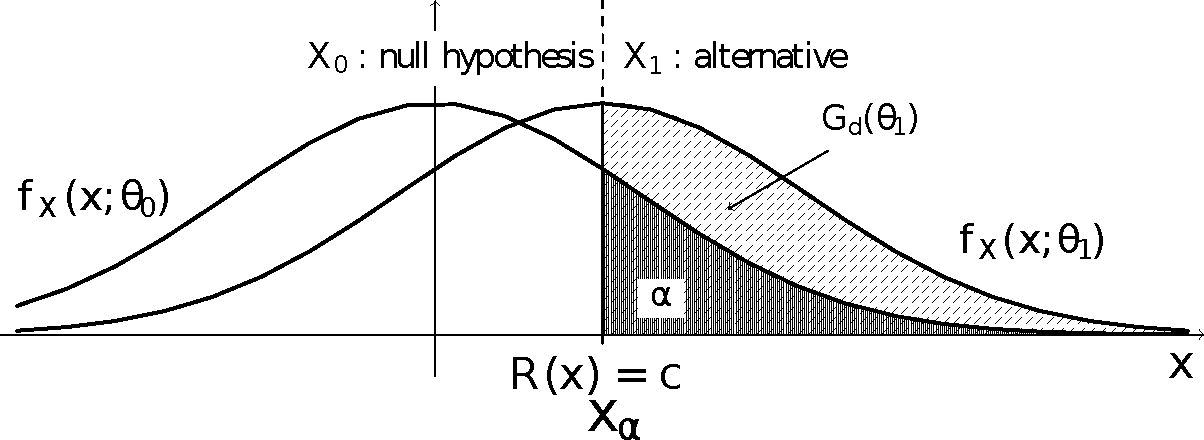
\includegraphics[width = \columnwidth]{tests}
	
	\textbf{Maximum Likelihood Detector:} \quad
	$T_{\ir ML}(x) = \begin{cases} 1 & R(x) > 1 \\ 0 & \text{otherwise} \end{cases}$\\
	\textbf{ROC Graphs:} plot $G_T(θ_1)$ as a function of $G_T(θ_0)$
\end{sectionbox}

\begin{sectionbox}
	\subsection{Bayes Test (MAP Test)}
	Prior knowledge about possible hypotheses:\\$\P(\{θ ∈ Θ_0 \}) + \P(\{θ ∈ Θ_1\}) =  1 $\\ 
	$T_{\ir Bayes} = \underset{T}{\operatorname{argmin}}\{P_{\epsilon}\}= 
	\begin{cases} 1 &;\quad\!\frac{f_{X}(x|θ_1)}{f_{X}(x|θ_0)} > c\\
	0&;\quad\text{otherwise}\end{cases} \\= \begin{cases} 1&;\quad \P(θ_1|x) > \P(θ_0|x) \\ 0 &;\quad \text{otherwise} \end{cases}\\
	\text{with}:\\ 
	P_{\epsilon} = P(\theta_0)G_T(\theta_0)+P(\theta_1)(1-G_T(\theta_1)),\quad c = \frac{P(\theta_0)}{P(\theta_1)}$\\\\
	\textbf{if} $P(\theta_0) = P(\theta_1) \implies T_{\ir Bayes} = T_{\ir ML}$\\\\
	\textbf{Multiple Hypothesis} $\{\theta_0,...,\theta_k\}; \mathbb{X}_0,...,\mathbb{X}_k \in \mathbb{X}$:\\
	$T_{\ir Bayes} = \underset{k\in1,...,K}{\operatorname{argmin}}\{P(\theta_k|x)\}$\\\\
	\textbf{Loss Function}:\\
	$L(T(x), θ) = \begin{cases} L_0 &;\quad T(x) = 1, \text{ but }θ = θ_0\quad \text{(FALSE ALARM)} \\
	L_1 &;\quad T(x) = 0, \text{ but }θ = θ_1\quad \text{(DETEC. ERROR)}\\
	0 &;\quad \text{otherwise} \end{cases}$\\
	$L_i$ denotes the Loss Value in cases where the correct decision parameter $θ_i$ is missed.\\
	$\operatorname{Risk}(T) = \E[L(T(\X), θ)] = \E [\E [L(T(x), θ)|x = \X ]]$\\
\end{sectionbox}

\begin{sectionbox}
	\subsection{Linear Alternative Tests}
	
	Estimate normal vector $\vec w^\top$ and $w_0$, which separate $\mathbb X$ into $\mathbb X_0$ and $\mathbb X_1$\\
	$\log R(\vec x) = -\frac{1}{2}\ln(\frac{\det(\ma C_1)}{\det(\ma C_0)}) - \frac{1}{2}(\vec x- \vec{μ}_1)^\top\ma C_1^{-1}(\vec x- \vec{μ}_1) +\\+\frac{1}{2}(\vec x- \vec{μ}_0)^\top\ma C_0^{-1}(\vec x- \vec{μ}_0) = \ln(\frac{P(\theta\in\Theta_0)}{P(\theta\in\Theta_1)})$ (seperating surface)\\\\
	For Gaussian $f_X(x; \mu_k, C_k)$ with $θ_0$ and $θ_1$ corresponding to $\{\mu_0,C_0\}$ and $\{\mu_1, C_1\}$, it follows that
	\begin{itemize}
		\item if $C_0 \ne C_1$, $logR(x) = 0$ is non-linear and the separating surfaces are surfaces of second order:
		parabolic, hyperbolic, or elliptic surfaces.
		\item if $C_0 = C_1$, $logR(x) = 0$ is affine and thus defines a hyperplane in $\mathbb{X}$ which decomposes $\mathbb{X}$ into $\mathbb{X}_0$ and $\mathbb{X}_1$, i.e.,\\
		$T: \mathbb X \ra \R, \vec x \mapsto \begin{cases} 1 & \vec w^\top \vec x > w_0\\ 0 & \text{otherwise}\end{cases}$\\
		\begin{itemize}
			\item case 1: $\ma C_0 = \ma C_1 = \sigma^2\ma I_N$\\
			$\vec w^\top = (\vec\mu_1-\vec\mu_0)^\top,\\
			w_0= \frac{1}{2}(\vec\mu_1^\top\vec\mu_1-\vec\mu_0^\top\vec\mu_0) -\sigma^2\ln(\frac{P(\theta\in\Theta_1)}{P(\theta\in\Theta_0)})$\\
			$\vec w$ colinear with $(\vec \mu_1-\vec \mu_0)\\\implies \text{hyperplane orthogonal to } (\vec \mu_1-\vec \mu_0)$ 
			\item case 2: $\ma C_0 = \ma C_1 = \ma C$\\
			$\vec w^\top = (\vec\mu_1-\vec\mu_0)^\top\ma C^{-1},\\
			w_0= \frac{1}{2}(\vec {μ}_1 - \vec{μ}_0)^\top \ma C^{-1} (\vec {μ}_1 + \vec{μ}_0) -	\ln(\frac{P(\theta\in\Theta_1)}{P(\theta\in\Theta_0)})$\\
			in general $\vec w$ \textbf{not} colinear with $(\vec \mu_1-\vec \mu_0)\\\implies \text{hyperplane \textbf{not} orthogonal to } (\vec \mu_1-\vec \mu_0)$ 
		\end{itemize}
		\item if $C_0 = C_1$ and $\mu_0 = −\mu_1$, $log R(x) = 0$ is linear and defines a separating hyperplane in $\mathbb{X}$ which contains the origin, i.e.,\\
		$T: \mathbb X \ra \R, \vec x \mapsto \begin{cases} 1 & \vec w^\top \vec x > 0\\ 0 & \text{otherwise}\end{cases}$\\
	\end{itemize}
	
	
	% Bild aus Part7 p 197!!!
	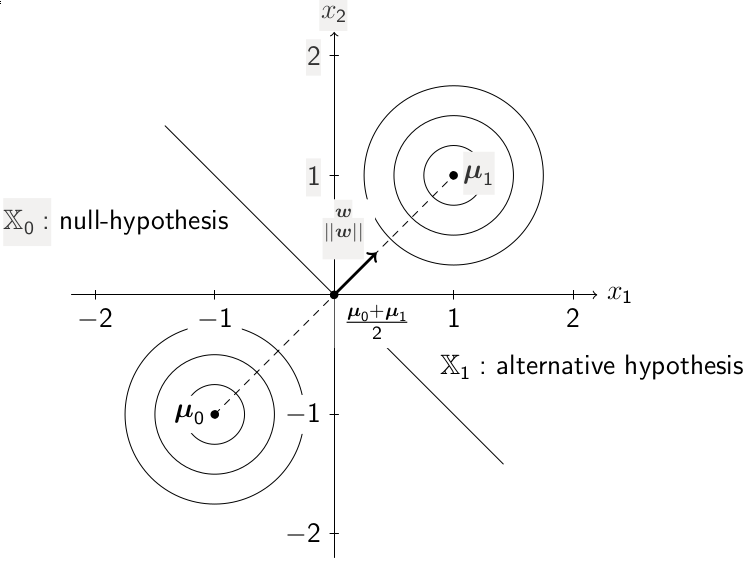
\includegraphics[width = \columnwidth]{linest2}
	
\end{sectionbox}

% Section
% ----------------------------------------------------------------------
\section{Hypothesis Testing}
making a decision based on the observations

\begin{sectionbox}
	\subsection{Definition}

	Null hypothesis $H_0: θ ∈ Θ_0$ (Assumed first to be true)\\
	Alternate hypothesis $H_1: θ ∈ Θ_1$ (The one to proof) \\
	Descision rule $φ: \mathbb X \ra [0, 1]$ with \\
	$φ(x) = 1$: decide for $H_1$, $φ(x) = 0$: decide for $H_0$
	Error level $α$ with $\E[d(\X)|θ] \le α, ∀θ∈Θ_0$

	\begin{tablebox}{p{7mm}llp{17mm}}
		Error Type & ${}_{\text{Decision}}$\!{\large $\diagdown$}\!${}^{\text{Reality}}$ & $H_1$ false {\small ($H_0$ true)} & $H_1$ true {\small ($H_0$ false)}
		\\ \cmrule
		1 (FA) False& $H_1$ rejected & \textbf{T}rue \textbf{N}egative & \textbf{F}alse \textbf{N}egative (Type 2)
		\\
		Alarm & \small ($H_0$ accepted) & $\P = 1-α$  & $\P = β$
		\\[1em]
		2 (DE) & $H_1$ accepted & \textbf{F}alse \textbf{P}ositive (Type 1) & \textbf{T}rue \textbf{P}ositive
		\\
		Detection Error & \small($H_0$ rejected) & $\P = α$ & $\P = 1-β$
	\end{tablebox}
	Power:
	Sensitivity/Recall/Hit Rate: $\frac{\text{TP}}{\text{TP}+\text{FN}}=1-β$\\
	Specificity/True negative rate: $\frac{\text{TN}}{\text{FP}+\text{TN}}=1-α$\\
	Precision/Positive Prediciton rate: $\frac{\text{TP}}{\text{TP}+\text{FP}}$\\
	Accuracy: $\frac{\text{TP} + \text{TN}}{\text{P}+\text{N}} = \frac{2-α-β}{2}$


	\subsubsection{Design of a test}
	Cost criterion $G_{φ}: Θ \ra [0, 1], θ \mapsto \E[d(X)|θ]$\\
	False Positive lower than $α$: $G_d(θ)|_{θ∈Θ_0} ≤ α, ∀ θ ∈ Θ_0$\\
	False Negative small as possible: $\max \{G_d(θ)|_{θ∈Θ_1}\}, ∀ θ ∈ Θ_1$
\end{sectionbox}



\begin{sectionbox}
	\subsection{Sufficient Statistics}
	Sufficiency for a test $T(\X)$ means that no other test statistic, i.e., function of the observations $\vec x$,
contains additional information about the parameter $θ$ to be estimated:\\
$f_{\X|T} (x|T(x) = t, θ) = f_{\X|T}(x|T (x) = t)$

\end{sectionbox}


\vfill

% Section
% ----------------------------------------------------------------------
\section{Support Vector Machines}

	\paragraph{Motivation and Background}
\begin{sectionbox}

	\subsection{Kernel Methods} 
	Kernel Methods is non-parametic estimation, these make no assumption on statistical model $\rightarrow$ purely Data-Based. \\
	\textbf{Test Statistic} 
	$\boxed{\mathbb{X} \rightarrow \mathbb{R}, \mathbf{x}\mapsto S(\mathbf{x})= \sum_{k=1}^{M} \lambda_kg(\mathbf{x}, \mathbf{\mu_k})}$ \\
	linear combination of Kernel Function $g(.,\mu_k)$, g() generally non-linear pos. definite \\ %TODO: besser einrichten
	
	$\mu_k$: representative for Sample Set $\mathbb{S}=\{x_1,...,x_M\}$ \\  
	$\lambda_k$: weight coefficient determined by learning \\
	Sample Set $\mathbb{S}$ is Empirical Characterization of Unknown Statistical Model \\
	Infernce of $\lambda_k$ based on Sample Set or Training Set is called \textbf{Learning}

	
\end{sectionbox}

\begin{sectionbox}
	\subsection{Kernel Tests}
Statistical Hypothesis Test decomposes sample space $\mathbb{X}$ into two disjoint subsets, the relative postion of a sample $x_j$ to the seperating surface \\determines choice of hypothesis\\
$\boxed{\mathbb{S} = \{(x_1, y_1),...,(x_M, y_M)\}}$ %TODO: Einrichten
\\
$x_i \in \mathbb{R}^N$, $y_i \in \{\Theta_0, \Theta_1\}$ \\
Inference of Hypothesis Test based on a Sample Set that includes Labeling $y_i$ of the elements $x_i$ is called \textbf{Supervised Learning} \\
$M \geq dim(\mathbb{X})$
\end{sectionbox}


\begin{sectionbox}
\subsection{Linear Kernels}
\textbf{Test Statistic} for linear test \\
$\boxed{S(x) = \sum_{i = 1}^{M}\lambda_i\mathbf{x_i}^T\mathbf{x} + wo = \mathbf{w}^T\mathbf{x} +wo}$ $\mathbf{w} = \sum_{i = 1}^{M}\lambda_ix_i$ \\
Hyperplane defined by $\mathbf{w}$(normal vector or weight vector) and $w_o$\\ approximates seperating surface between $\mathbb{X_-}$ and $\mathbb{X_+}$, therefor \\
$\boxed{T(\mathbf{x}) = sign(S(\mathbf{x})) = \begin{cases} 
			+1&;\quad \mathbf{w}^T\mathbf{x} +wo \geq 0\\
	        -1&;\quad otherwise
	\end{cases}}$\\ 
%TODO: insert illustration of linear kernel test
To determine $\mathbf{w}$ and $w_0$ formulate problem as constrained optimaization problem with the constraints: \\
$\forall k\in \{1,...M\}:T(\mathbf{x}_k)= y_k$ \\
$\Rightarrow$ \textbf{Support Vector Methods}:$\boxed{y_k(\mathbf{w}^T\mathbf{x}_k+wo)\geq \epsilon, \forall k}$ \begin{flushright}maximize margin $\epsilon$ for constant norm of $\mathbf{w}$ \end{flushright} 

\end{sectionbox}

\paragraph{Application}
\begin{sectionbox}
	
\subsection{Support Vector Methods}
only feasible for normalized weight vectors \\
%{0 \leq q \leq n-1}} f(q) \le n$,
$\smash{\displaystyle\max_{w}}$ $\epsilon$  s.t.  $y_k \frac{\mathbf{w}^T}{\norm{\mathbf{w}}_2}\mathbf{x}_k \geq \epsilon, \forall k$ , $w_0 = 0$\\ 
$\Leftrightarrow$\hspace{1pt} $\smash{\displaystyle\min_{w}}$ $\frac{1}{2}\norm{\mathbf{w}}_{2}^{2}$ s.t. $y_k\mathbf{w}^T\mathbf{x}_k \geq1, \forall k$ \\
Optimization Problem convex $\rightarrow$ \textbf{Langragian Method} \\ \\
Dual Problem: $\smash{\displaystyle\max_{\mathbf{u}}}$$\smash{\displaystyle\min_{\mathbf{w}}}$ $\Phi (\mathbf{w}, \mathbf{u})$ s.t. $\mathbf{u} \geq 0$ \\ \\
Langragian Multiplier: $u_k \geq 0$   \\
Langragian Fct: $\Phi (\mathbf{w}, \mathbf{u}) = \frac{1}{2}\mathbf{w}^T\mathbf{w} +\sum_{k=1}^{M}u_k(1-y_k\mathbf{w}^T\mathbf{x_k})$  \\
$\frac{\partial\Phi (\mathbf{w}, \mathbf{u})}{\partial\mathbf{w}}|\begin{tiny}_
{\mathbf{w}=\mathbf{w(\mathbf{u})}}.
\end{tiny} = 0$\hspace{1pt} $\leftrightarrow$ \hspace{1pt} $\mathbf{w}(\mathbf{u}) = \sum_{k=1}^{M}\underbrace{u_ky_k}_{\lambda_{k}}\mathbf{x_k}$

Evaluate dual function: \\
$\Phi(\mathbf{w(\mathbf{u})}, \mathbf{u}) = \Phi(\sum_{k=1}^{M}u_ky_k\mathbf{x}_k, u_1...,u_M) \\
= -\frac{1}{2}\sum_{k=1}^{M}\sum_{l=1}^{M}u_ku_ly_ky_l\mathbf{x}_k^T\mathbf{x}_l + \sum_{k=1}^{M}u_k \\
= -\frac{1}{2}\mathbf{u^T}\mathbf{YXX^TYu}+\mathbf{1^Tu} \\
\mathbf{X}= \begin{bmatrix}
\mathbf{x_1^T} \\
\vdots \\
\mathbf{x_M^T}
\end{bmatrix}, \mathbf{Y} =\begin{bmatrix}
y_1 & & \\
&\ddots &\\
& & y_M
\end{bmatrix}, \mathbf{1} = \begin{bmatrix}
 1\\
 \vdots\\
 1
\end{bmatrix} $
%TODO: insert interative solution?


\end{sectionbox}
\begin{sectionbox}
	\subsection{Suport Vectors}
	Dual OP.:$\smash{\displaystyle\max_{\mathbf{u}}}$  $\sum_{k=1}^{M}(-\frac{1}{2}\sum_{l=1}^{M}u_ku_ly_ky_l\mathbf{x_k^Tx_l}+u_k)$s.t.$u_k\geq0$ \\\\
	\textbf{Optimal Dual Variables} $u_1^*,...,u_M^*$ either \textbf{active} $u_k>0$ \\or \textbf{inactive} $u_k=0$ \\
	Elements of $\mathbb{S}$ with active dual variables = \textbf{Support Vectors} 
	$\boxed{\mathbb{S}_{\tiny{SV}}=\{ \mathbf{x}_k \in \mathbb{S}|u_k^* >0\}}$\\
	Elements with inactive dual variables %\begin{flushright
	dont contribute to Kernel Test \\
	\textbf{Optimal Weight Vektor} $\mathbf{w^*} = \mathbf{w(u^*)}$ of Kernel Test constructed by Support Vectors only: 
	$\boxed{\mathbf{w^*}=\sum_{\mathbf{x}_k\in\mathbb{S}_{SV}} u_k^*y_k\mathbf{x}_k}$ \\
	Number of Support Vectors approx. size of dim$[\mathbb{X}]$ $\rightarrow$ selection of Support Vectors reduces computational complexity of Kernel Test
	%TODO: insert geometric interpretation
	\paragraph{Discussion}
	\begin{itemize}
		\item Exists only if $\mathbb{S} $ \textbf{Linearly Separable}
		\item $w_0 \neq 0$ no (straightforward) iterative solution available
		\item if \textbf{Linearly Inseperable} method generalized by slack variables for controlled violation of constraints 
	\end{itemize}
	
\end{sectionbox}

\begin{sectionbox}
	\subsection{Kernel Trick}
	\textbf{Linear Hypothesis Test} often not sufficient: \textbf{Kernel Trick}: Generalize linear methods to non-linear approximation of seperating surfaces $(\{x|\log R(\mathbf{x})=c\})$ \\
	Basic Idea: Transfer problem statement into higher-dimensional space(without introducing additional degrees of freedom) by \textbf{Feature Map} $\varphi: \mathbb{S}\rightarrow\mathbb{S}_{\varphi}$
\end{sectionbox}	--

% Section
% ----------------------------------------------------------------------
\section{Learning and Generalization}

\begin{sectionbox}
	\subsection{Empirical Risk Function and Generalization Error}
	ML scenarios (unknown Stochastical Model) base learning on:
	$Risk_{emp}(T;\mathbb{S})=\frac{1}{M}\sum_{i=1}^{M}L(T(\vx_i),y_i),\quad(\vx_i,y_i)\in\mathbb{S}$
	
	$\vx\mapsto T(\vx;\mathbb{S})\quad T=\underset{T'\in\mathbb{T}}{\operatorname{argmin}}\{Risk_{emp}(T';\mathbb{S})\}$
	
	\textbf{good Generalization}: $Risk_{emp}(T;\mathbb{S}_{test})$ similar to $Risk_{emp}(T;\mathbb{S})$ 
	\textbf{bad Generalization}:
	\begin{itemize}
		\item small $\mathbb{T}$ that does not cover $T_{opt}$ $\rightarrow$ cannot be selected by ML
	\end{itemize}
	$\Rightarrow$ strong mismatch between the desired and derived \textit{Test} and refers to a sort of \textit{Bias Error Term}
	\begin{itemize}
		\item too rich $\mathbb{T}$ $\rightarrow$ fluctuating of the available data (measurement noise) is interpreted as meaningful information
	\end{itemize}
	$\Rightarrow$ \textit{Overfitting}; leads to an increased \textit{Variance Error Term}
	
\end{sectionbox}

\begin{sectionbox}
	\subsection{Bias-Variance Decomposition}
	$Risk=E_{S,X,Y}[L(T(X;S),Y)]=E_X[1-P_{Y|X}(Y=T_B(X))+(1-P_{S|X}(T(X;S)=T_B(X)))(2P_{Y|X}(Y=T_B(X))-1)],\quad T_B(X)$ is the unknown \textit{Bayes Test}
	
	If the potential set $\mathbb{S}$ would be selected from a distribution such that the derived Test $T(\vx; \mathbb{S})$ and the corresponding Bayes Test $T_B(\vx)$ are identical almost surely, then the Risk Function achieves its minimum value which is equal to the \textit{Irreducible Error} $E_X[1 − P_{Y|X}(Y = T_B(X))]$(denotes the probability that for a given input $\vx$ the Bayes Test $T_B(X)$
	decides for the false label $y$).
	
\end{sectionbox}

% Section
% ----------------------------------------------------------------------
\section{Classification Trees and Random Forests}

\begin{sectionbox}
	\subsection{CART Algorithms}
	
\end{sectionbox}

\begin{sectionbox}
	\subsection{Random Forests}	
	
\end{sectionbox}


% Section
% ----------------------------------------------------------------------

\section{Deep Neural Networks}
\begin{sectionbox}
\subsection{From Kernel to Neural Networks (NN)}
NN: methodology by which KERNELS are determined by chosen learning method based on the available training data $\rightarrow$ KERNELS are composed by a concatenation of multiple VECTOR VALUED functions
\begin{emphbox}
$g(x)=f^{(L)}(f^{(L-1)}(...f^{(2)}(f^{(1)}(x;W^{(1)},v^{(1)});$\\
$W^{(2)},v^{(2)})...;W^{(L-1)},v^{(L-1)});W^{(L)},v^{(L)})$
\end{emphbox}
$f^{(l)}(*;W^{(l)},v^{(l)})\in \R^{N_t}$ represents the l-th layer of NN\\
NN consist of L+2 layers (INPUT Layer $x \in \R^N$ and LAYER OF OUTPUTS $f^{(NN)}\in \R^{N_{L+1}}$\\
HIDDEN LAYER (L=1) often enough\\
If $L>1$ NN is called \textbf{DEEP}\\

Mapping between NN layers consists typically of AFFINE TRANSFORMATION of the output of the preceding layer;\\
$\R^{N_{t-1}}\rightarrow \R{N_t}:f^{(l-1)} \rightarrow^{(l)}=W^{(l),T}f^{(l-1)}+v{(l)}$,\\
and the elementwise NONLINEAR TRANSFORMATION of the resulting INTERNAL STATE VECTOR $z^{(l)}$ by means of a NONLINEAR FUNCTION $\sigma^{(l)}$\\

\begin{emphbox}
$f^{(l)}(f^{(l-1)};W^{l}),v^{(l)})=\sigma^{(l)}(W^{(l),T}f^{(l-1)}+v^{(l)})$
\end{emphbox}

Elements of $^{(l)}$ and $v^{(l)}$ are called weights of the lth NN layer
\begin{itemize}
\item INPUT LAYER (l=0) of NN equals INPUT VECTOR $x \in \R^N$
\item OUTPUT LAYER (l=L+1) of NN equals OUTPUT VECTOR $f^{(NN)}\in \R^{N_{L+1}}$
\item NONLINEAR FUNCTION $\sigma_i^{(l)}$ of the HIDDEN LAYERS is different from the OUTPUT FUNCTION of the OUTPUT LAYER
\item latter depends on LOSS FUNCTION and the chosen LEARNING ALGORITHM
\end{itemize}

Single nonlinear function of the output vector of the previous layer composed by the i-th LINEAR FUNCTIONAL $w_i^{(l)}$, the CONSTANT $v_i^{(l)}$ and the i-th nonlinear function $\sigma^{(l)}$ of the next layer = NEURON. WEIGHTS represent the SYNAPTIC STRENGHTS and the nonlinear function $\sigma_i^{(l)}$ = ACTIVATION FUNCTION\\

\begin{emphbox}
$\sigma_i^{(l)}(\sum_{j=1}^{N_{(l-1)}}w_{i,j}^{(l)}f_j^{(l-1)}+v_i^{(l)})$
\end{emphbox}

\end{sectionbox}
\begin{sectionbox}

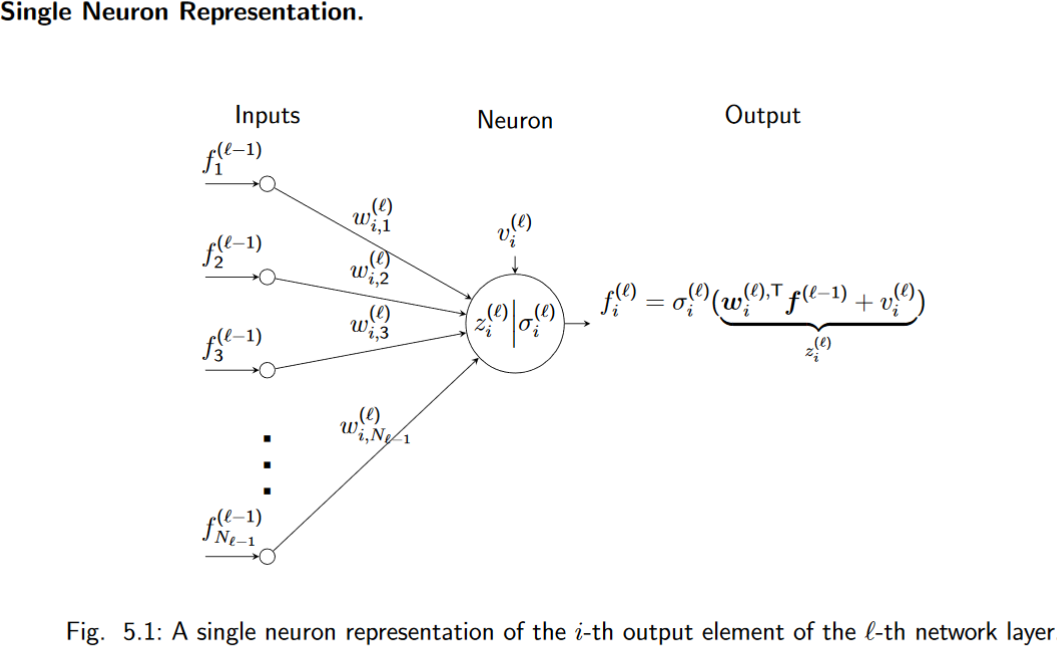
\includegraphics[width = \columnwidth]{./img/signalneuronrep}
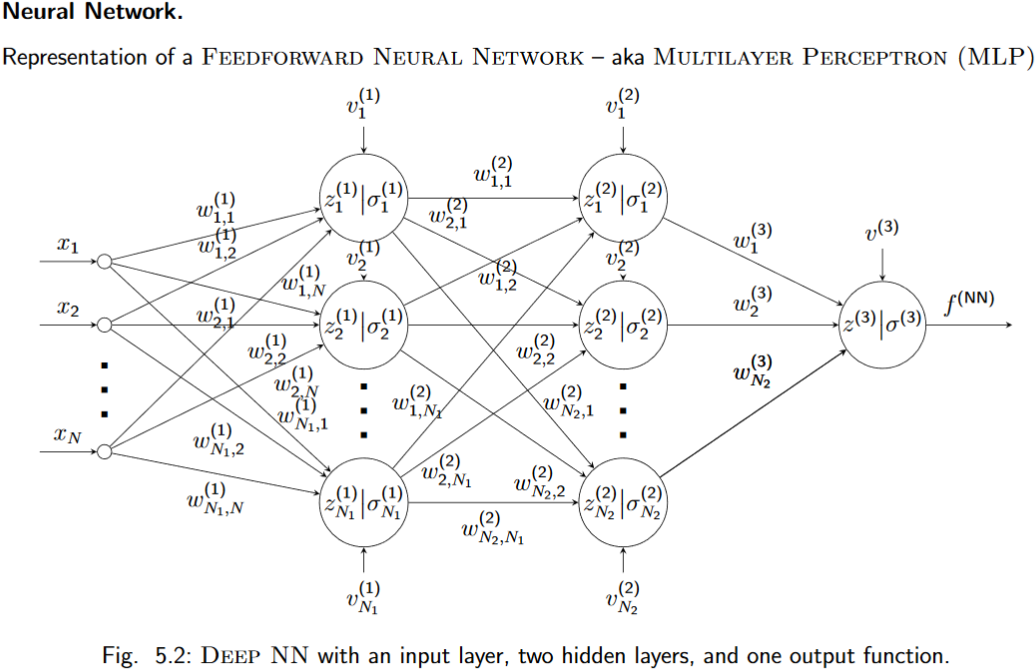
\includegraphics[width = \columnwidth]{./img/neuralnetwork}

\end{sectionbox}

\begin{sectionbox}
\subsection{Activation Functions}
\subsubsection*{ReLU Activation Functions}
most popular chose for the activation function$\sigma_i^{(l)}\rightarrow$ RECTIFIED LINEAR UNIT FUNCTION (RELU)\\

\begin{emphbox}
$\sigma(z_i^{(l)})=max(0,z_i^{(l)})\in \R_+$\\
with $z_i{(l)}=\sum_{j=1}^{N_{l-1}}w_{i,j}^{(l)}f_j^{(l-1)}+v_i^{(l)}$
\end{emphbox}

\begin{itemize}
\item PIECEWISE LINEAR FUNCTION which is zero for a negative state variable
\item efficient for the training of network weights, since its gradient with respect to the weight parameters does not experience any saturation for large positive values of the state variable, i.e.
\end{itemize}

\begin{emphbox}
$\frac{\partial \sigma(z_i^{(l)})}{\partial w_{i,j}^{(l)}}=\frac{\partial\sigma(z_i^{(l)})}{\partial z_i^{(l)}}\frac{\partial z_i^{(l)}}{\partial w_{i,j}^{(l)}}=unit(z_i^{(l)}f_j^{(l-1)})$ and\\
$\frac{\partial \sigma(z_i^{(l)})}{\partial v_{i,j}^{(l)}}=\frac{\partial\sigma(z_i^{(l)})}{\partial z_i^{(l)}}\frac{\partial z_i^{(l)}}{\partial v_{i,j}^{(l)}}=unit(z_i^{(l)})$\\
with the UNIT STEP FUNCTION unit(z)$\in{0,1}$
\end{emphbox}

%\parbox{5.5cm}{\emph{RELU AF:}\\ 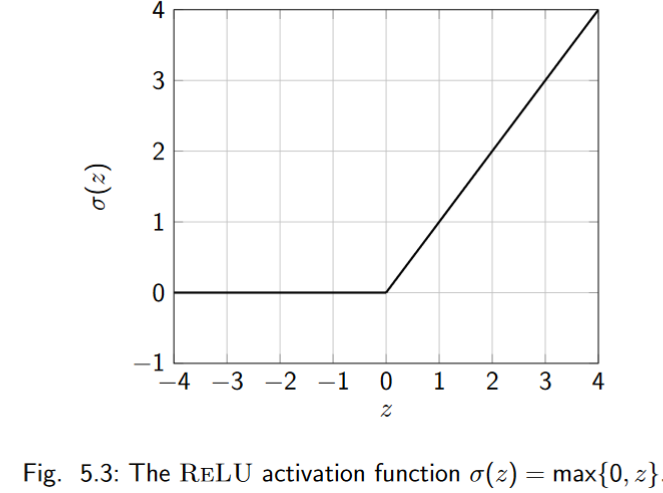
\includegraphics[width = 5.5cm]{./img/relu_af}}

\end{sectionbox}

\begin{sectionbox}
\subsubsection*{Hyperbolic Tangent Activation Functions}
Used to be standard before RELU
\begin{emphbox}
$ \sigma(z_i^{(l)})=tanh(z_i^{(l)})=\frac{e^{z_i^{(l)}}-e^{-z_i^{(l)}}}{e^{z_i^{(l)}}+e^{-z_i^{(l)}}} \in [-1,+1]$\\
with $z_i^{(l)}=\sum_{j=1}^{N_{l-1}}w_{i,j}^{(l)}f_j^{(l-1)}+v_i^{(l)}$
\end{emphbox}
The HYPERBOLIC TANGENT FUNCTION suffers from a saturation of its gradient with respect to weight parameters for large absolute values of the state variable, i.e.
\begin{emphbox}
$\frac{\partial \omega(z_i^{(l)})}{\partial w_{i,j}^{(l)}}=\frac{\partial\omega(z_i^{(l)})}{\partial z_i^{(l)}}\frac{\partial z_i^{(l)}}{\partial w_{i,j}^{(l)}}=(1-tanh^2(z_i^{(l)}))f_j^{(l-1)}$and\\
$\frac{\partial \omega(z_i^{(l)})}{\partial v_{i}^{(l)}}=(1-tanh^2(z_i^{(l)}))$
\end{emphbox}
Advantage: for small values of the state variable near $z_i^{(l)}=0$ the HYPERBOLIC TANGENT FUNCTION resembles a LINEAR MODEL\\

HYPERBOLIC TANGENT FUNCTION is very similiar to s.c. SIGMOID FUNCTION $\omega_{SIGMOID}(z_i^{(l)})=\frac{1}{1+e^{-z_i^{(l)}}}$\\
$\rightarrow tanh(z_i^{(l)})=2\sigma_{SIGMOID}(2z_i^{(l)})-1$\\

%\parbox{5.5cm}{\emph{Hyperbolic Tangent AF:}\\ 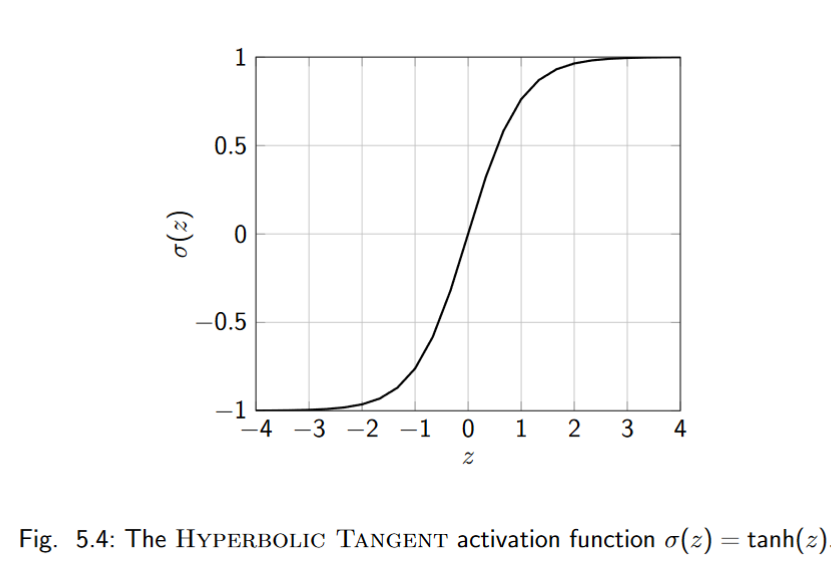
\includegraphics[width = 5.5cm]{./img/hyperbolic_tangent_af}}
%\parbox{5.5cm}{\emph{Sigmoid AF:}\\ 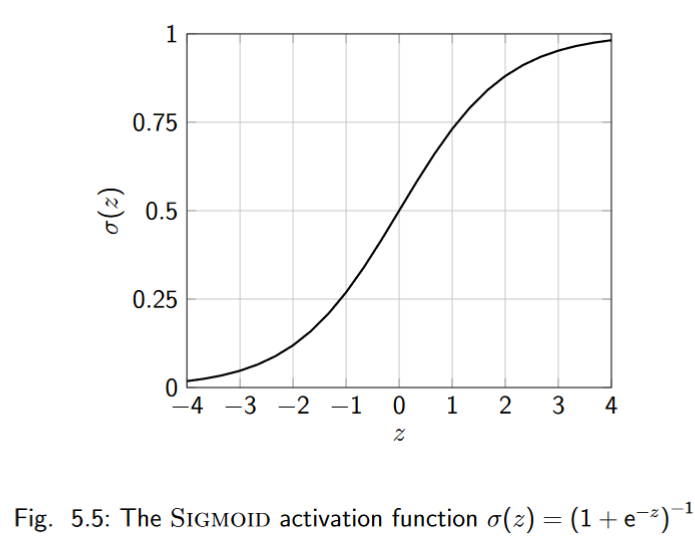
\includegraphics[width = 5.5cm]{./img/sigmoid_af}}
\end{sectionbox}







% ======================================================================
% End
% ======================================================================
\end{document}
